\chapter{Results and Discussion}
\section{Training Results}
The model was trained for 100 epochs, with early stopping triggered after 35 epochs. The final performance metrics on the validation set are summarized in Table \ref{tab:metrics}. The training progress, including loss curves and mean Average Precision (mAP), can be seen in Figure \ref{fig:results_graph}.

\begin{table}[H]
\centering
\begin{tabular}{|l|c|}
\hline
\textbf{Metric} & \textbf{Value} \\
\hline
mAP50-95 (mean Average Precision) & 0.756 \\
Precision & 0.963 \\
Recall & 0.958 \\
\hline
\end{tabular}
\caption{Model Performance Metrics on Validation Set.}
\label{tab:metrics}
\end{table}

\begin{figure}[H]
    \centering
    % NOTE: Make sure 'results.png' is in an accessible folder
    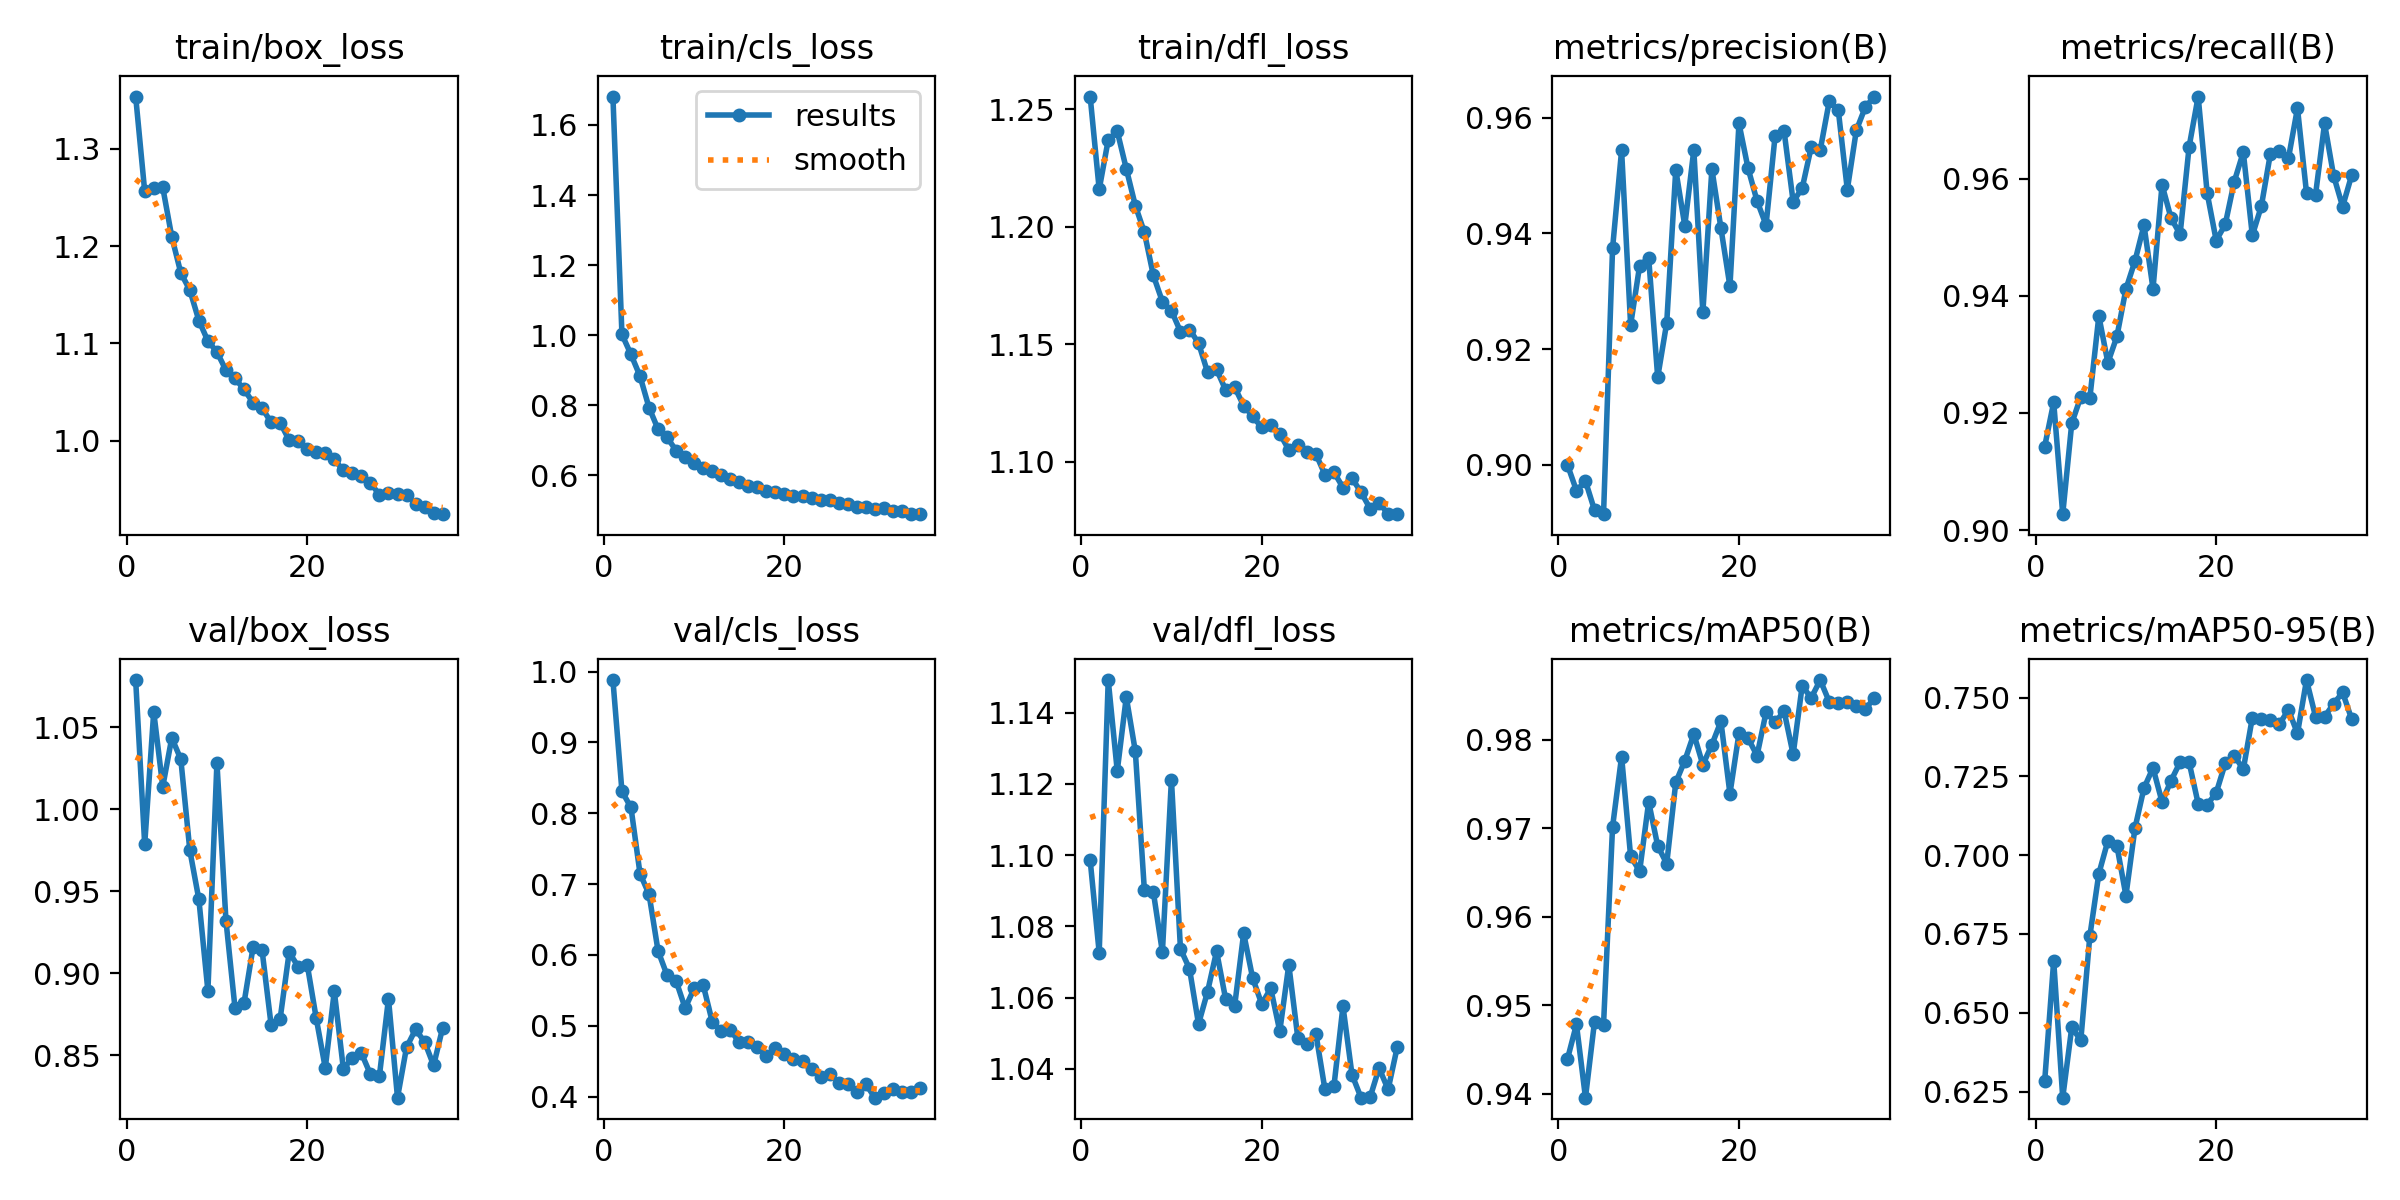
\includegraphics[width=0.9\textwidth]{../runs/detect/helmet_detection/results.png}
    \caption{Training performance graphs showing loss and mAP curves.}
    \label{fig:results_graph}
\end{figure}

The confusion matrix in Figure \ref{fig:confusion_matrix} further illustrates the model's performance. The diagonal represents correct classifications.

\begin{figure}[H]
    \centering
    % NOTE: Make sure 'confusion_matrix_normalized.png' is in an accessible folder
    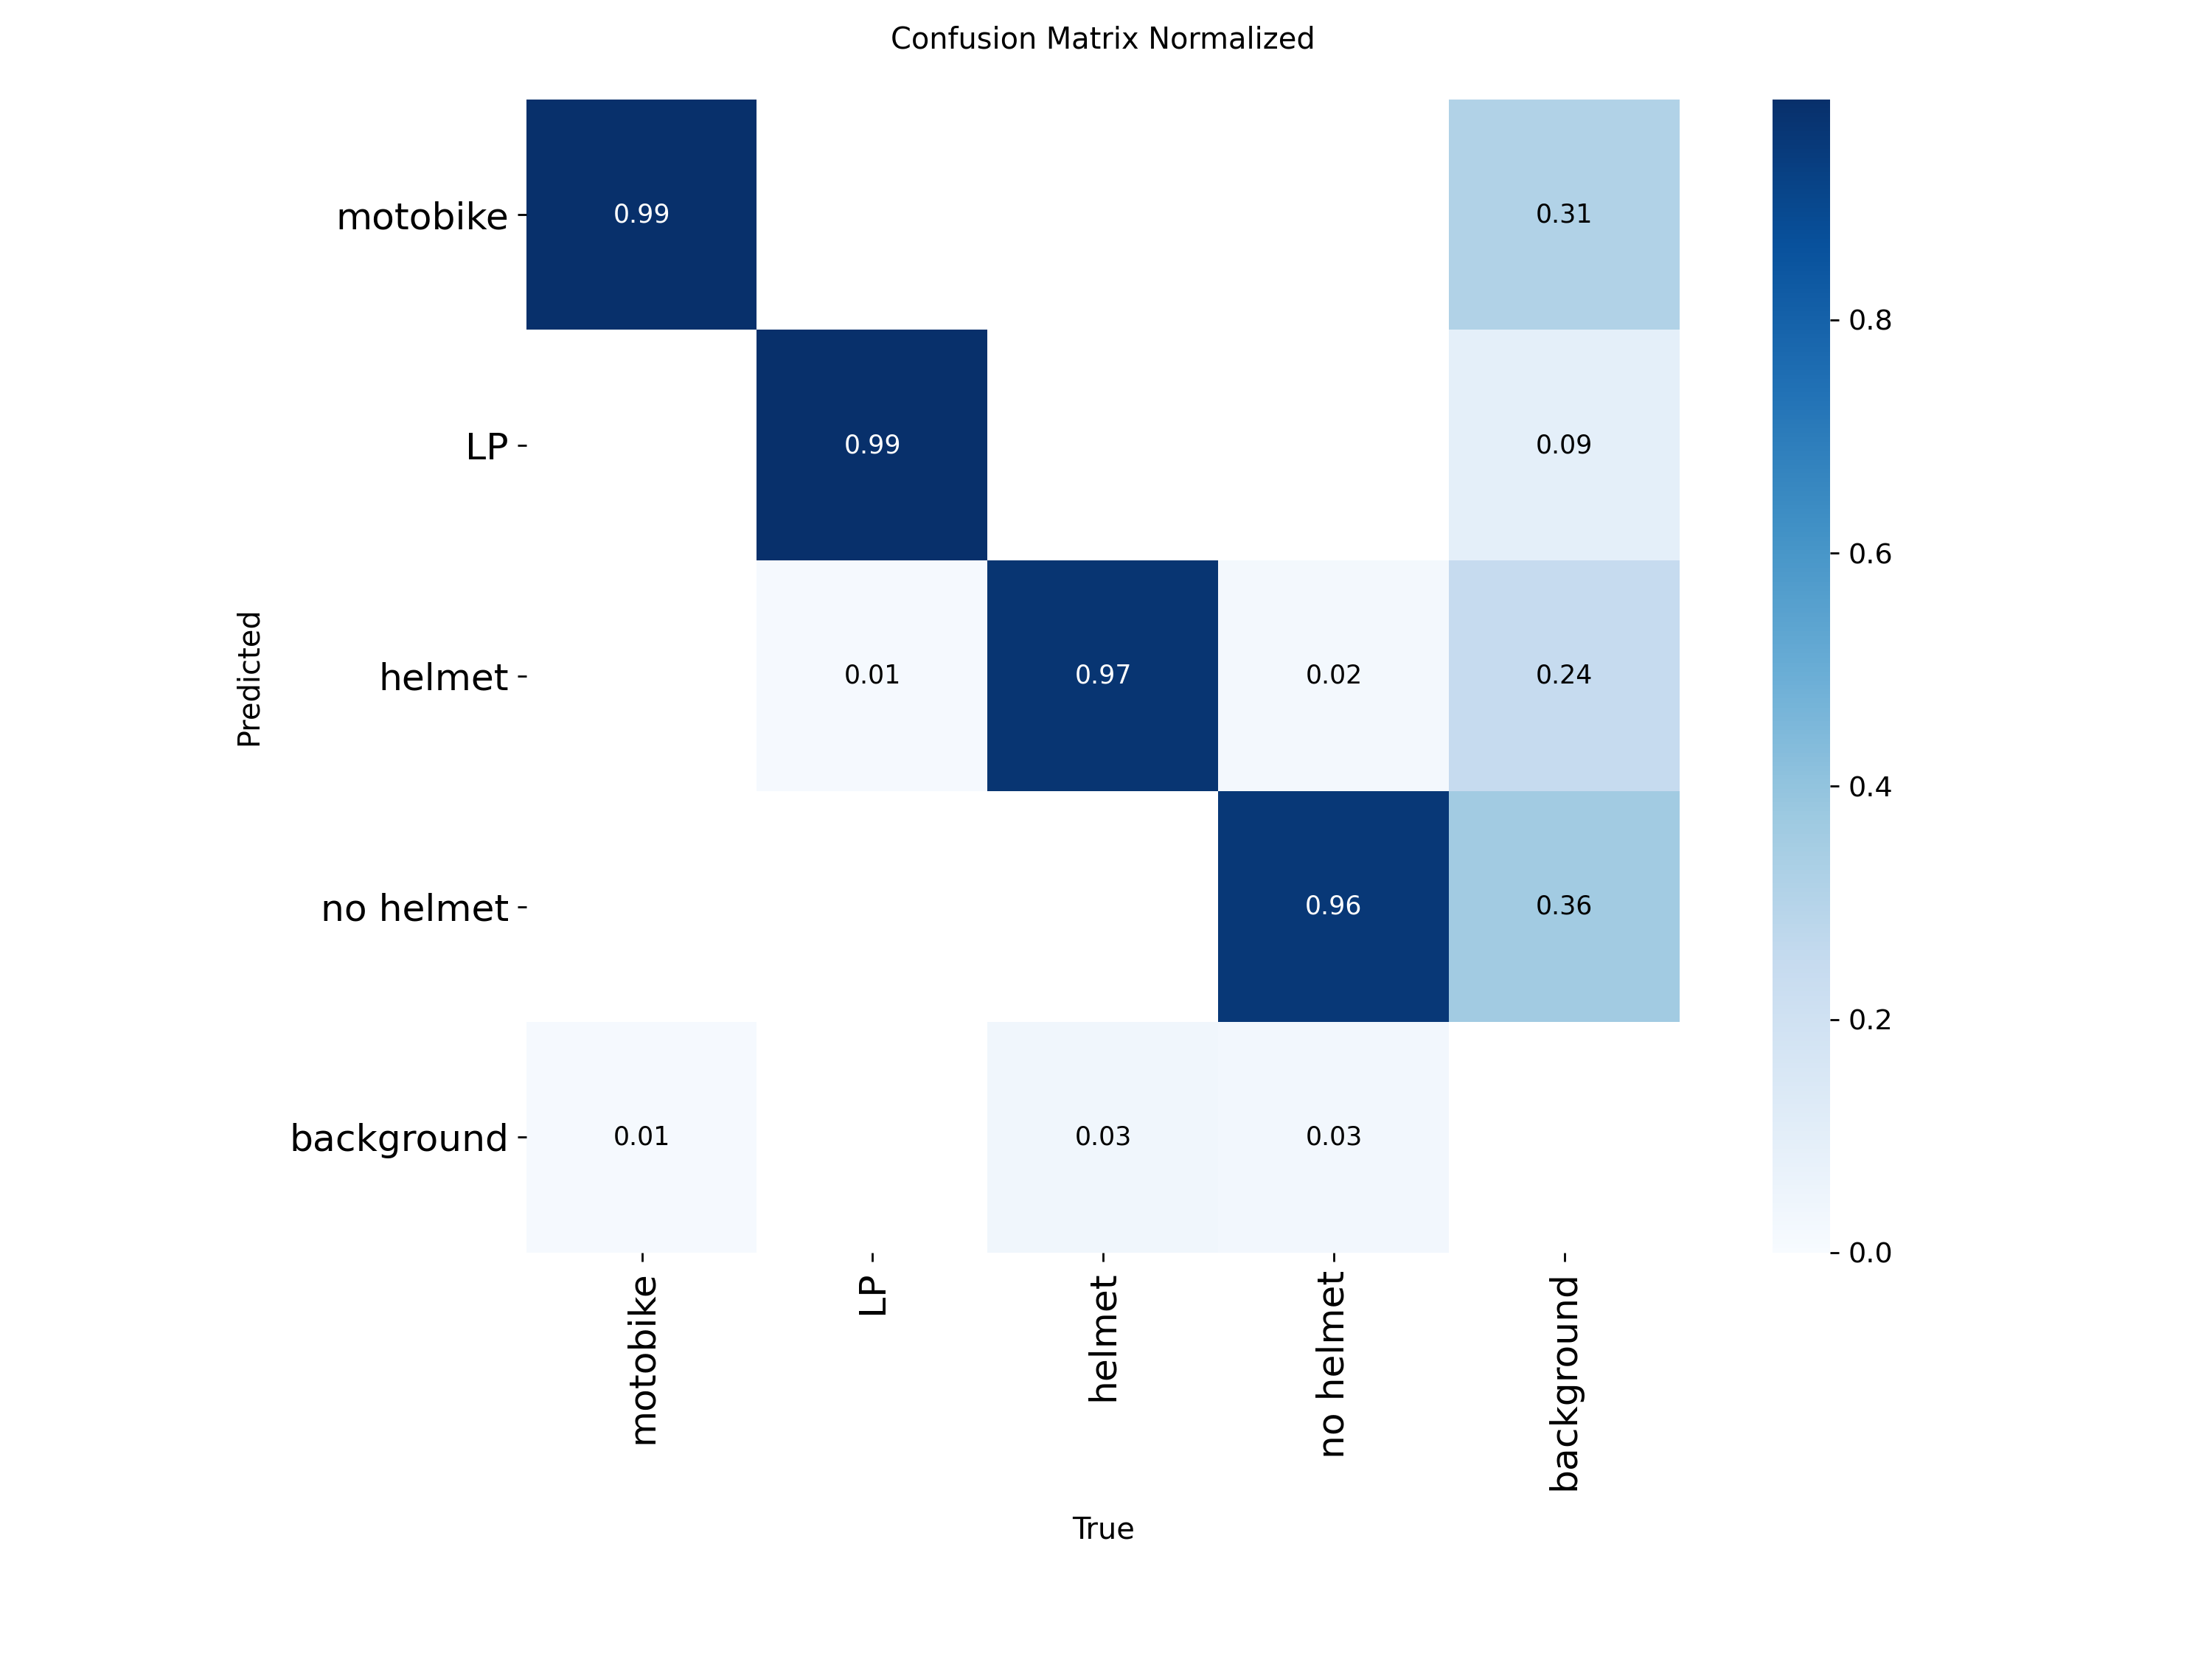
\includegraphics[width=1\textwidth]{../runs/detect/helmet_detection/confusion_matrix_normalized.png}
    \caption{Normalized confusion matrix for the validation set.}
    \label{fig:confusion_matrix}
\end{figure}

\section{Inference Performance on Raspberry Pi}
Using the \texttt{best\_float16.tflite} model, the average inference time per 320x320 image was approximately \textbf{850} milliseconds.

\section{Qualitative Results}
Figure \ref{fig:qualitative_results} shows an example of the model's predictions on a validation batch.

\begin{figure}[H]
    \centering
    % NOTE: Make sure 'val_batch0_pred.jpg' is in an accessible folder
    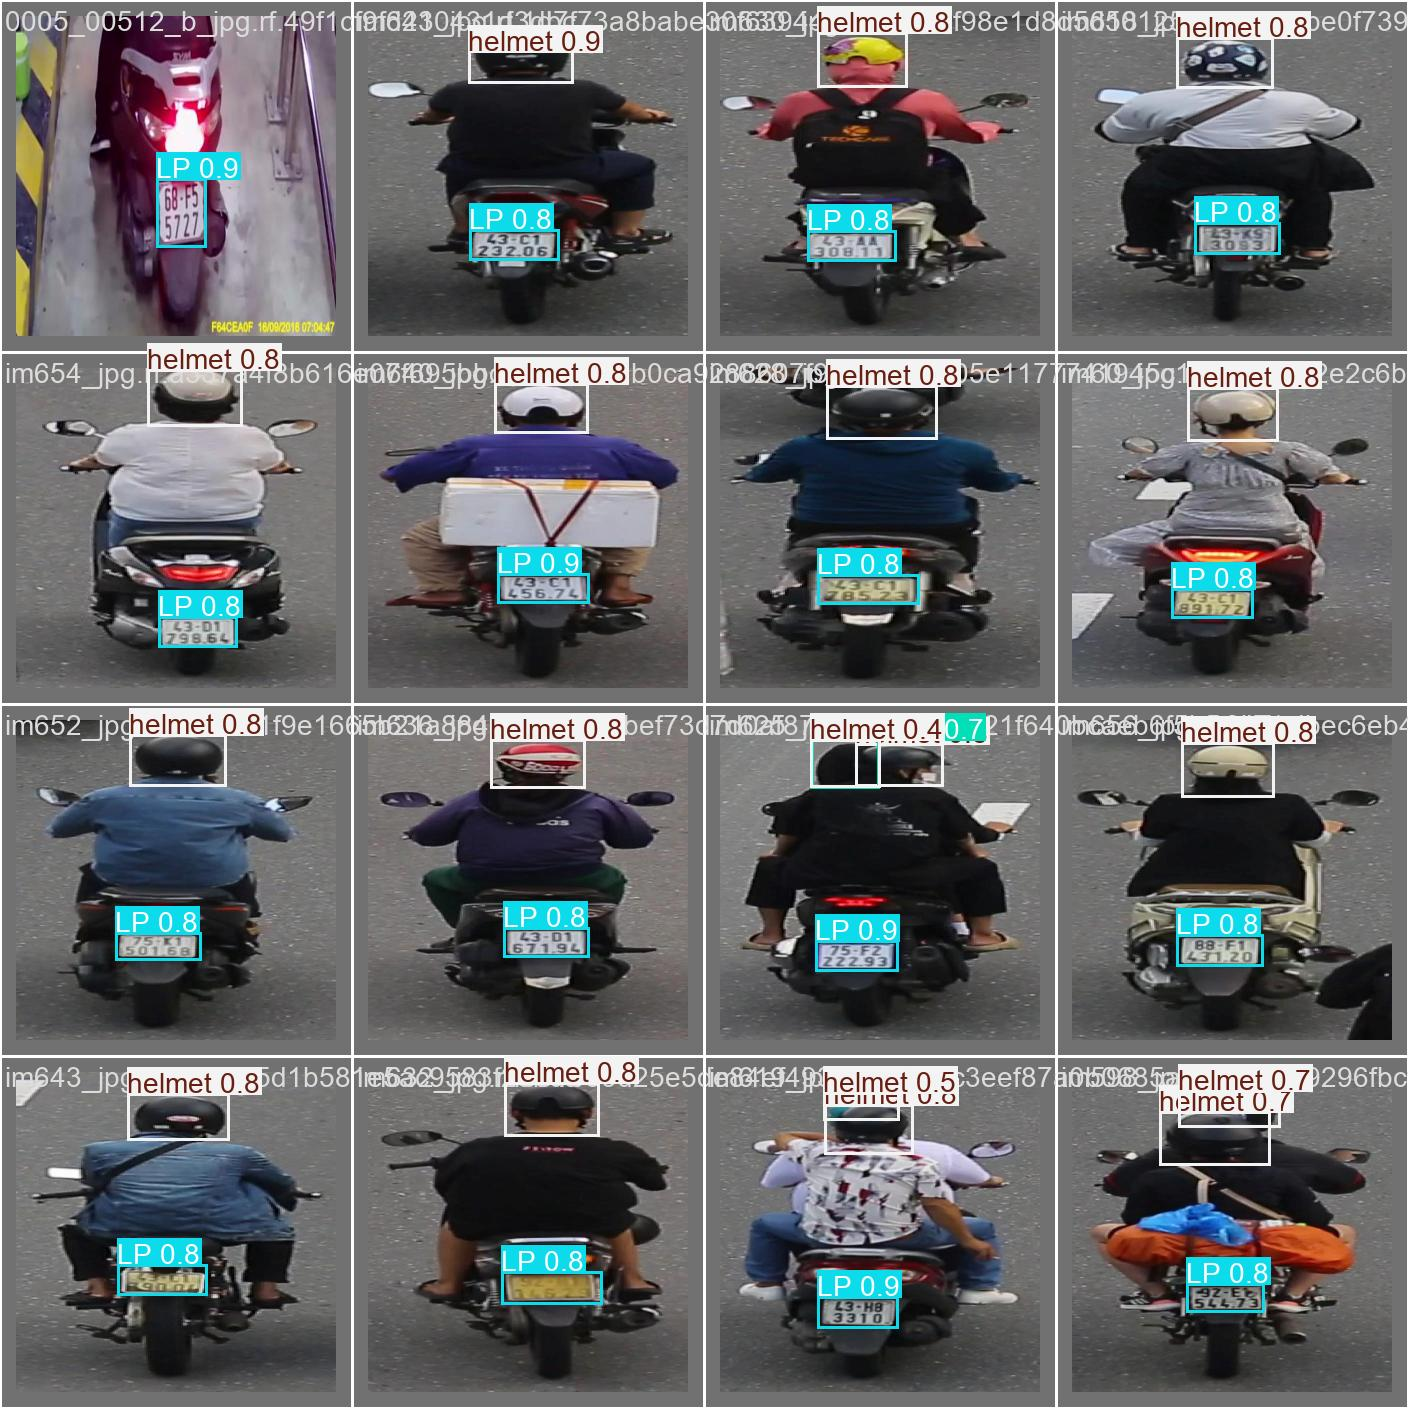
\includegraphics[width=0.8\textwidth]{../runs/detect/helmet_detection/val_batch0_pred.jpg}
    \caption{Qualitative detection results on a validation batch.}
    \label{fig:qualitative_results}
\end{figure}

\section{Discussion}
The results demonstrate that the YOLOv8n model, when properly optimized, is capable of performing effectively on the Raspberry Pi 3B+. The FP16 quantization was crucial in achieving an acceptable inference speed. However, some limitations were observed, such as difficulty with poorly lit images, motion blur, and very small objects.
